\chapter{Experiments and Results}\label{experiments}
% Structure:
%  - Intro: outline of chapter
%  - Models
%     - OOD testing, variance testing, (parameter count analysis)
%  - Augmentation Strategies
%     - No augmentation v Vanilla augmentations v gan augmentations
%  - Consistency loss vs normal loss
%  - Ensemble vs No ensemble
%  - Conclusion
%     Best pipeline vs baselines


\section{Metrics}
    %Intro here
    \subsection{IoU}
    The most natural way to quantify generalizability is to simply evaluate the predictors on in-distribution and out-of-distribution data, then consider the differences. There are, naturally, several performance measures that can be used to this end in the context of segmentation, the most natural being IoU or the Dice coefficient, which as discussed in Chapter \ref{background} are equivalent. In this thesis, IoU was used. To reiterate, IoU is defned as follows:
    Let \(y\) be the segmentation label, and \(\hat{y}=f(x)\) be the segmentation prediction given the model \(f\) and an input image x. The \gls{iou} can then be expressed as: 
    \begin{equation*}
        IoU(y, \hat{y}) = \frac{\sum \{y=\hat{y}\} }{\sum \{y=1\} \cup \{\hat{y}=1\}\}}
    \end{equation*}
    
    To evaluate the performance and generalziability of a predictor, IoU scores will be computed for each of the aforementioned datasets for every predictor. The mean \gls{iou} will then be calculated from the ten predictor samples. 
    
    However, since the predictors can vary considerably in performance also in the \gls{ind} case, it is necessary to consider the generalizability gaps as a percentage. This is computed as follows:
    \begin{equation}
        \Delta\%IoU = \frac{IoU_{ind}-IoU_{ood}}{IoU_{ind}}
    \end{equation}
    
    \subsection{SIS and SIS-AUC}
    As discussed in previous chapters, it is not necessarily the case that \gls{ood} datasets are available, hence the need for a validation procedure that can operate on \gls{ind} data but nevertheless presents some indication of the generalizability of the predictor. To this end, \gls{sis} may be used. SIS is, however, dependent on the perturbation model and the severity of the chosen augmentations. IN DEPTH EXPLANATION OF WHY AUC IS REQUIRED HERE 

\section{Datasets}
Naturally, the best way to evaluate the generalizability of a given predictor is to test it on out-of-distribution data. To achieve this, multiple datasets are required. \autoref{tab:datasets} shows the size, image resolutions and availability of the respective datasets used in this thesis.

\begin{table}[h]
    \centering
   \begin{tabularx}{\linewidth}{XXXX}
    \toprule
    Dataset & Resolution & Size & Availability \\
    \midrule
    Kvasir-Seg \cite{kvasir} & Variable & 1000 & Public \\
    Etis-LaribDB & 1255x966 & 196  & Public \\
    CVC-ClinicDB & 388x288 & 612  & Public \\
    EndocCV2020 & ? & ?  & Request \\
    \bottomrule
\end{tabularx}
    \caption{Dataset Overview}
    \label{tab:datasets}
\end{table}

% EndoCV2021 should also have been included, ideally, for better comparison to the results published in their proceedings, however since this dataset was unavailable at the time of writing this thesis, this was, unfortunately, not possible. 

Kvasir-SEG was used as the \gls{ind} dataset across all experiments due to its size and the diversity of images. The remaining datasets were used solely for \gls{ood} evaluation. 

\section{Models}
In order to evaluate the impact of the methods sufficiently, they need to be tested across a range of different models, namely DeepLabV3+, \gls{fpn}, UNet, Tri-Unet, and the dual-decoder DeepLabV3+ as introduced in Chapter \ref{methods}. This is intended to be a somewhat representative sample of "typical" deep learning pipelines, with a range of architectures and parameter counts. 
        
The models were implemented in pytorch using the segmentation-models-pytorch library \cite{smp}. The models were all implemented using the library's default values. \autoref{tab:models} shows the architecture type and parameter counts of the respective models. 
  \begin{table}[h]
            \centering
            \begin{tabularx}{\linewidth}{lXr}
            \toprule
                 Model & Architecture & Parameters  \\
            \midrule
                 UNet & Encoder-Decoder & 0\\ 
                 TriUnet & Stacked Encoder-Decoder & 0\\
                 FPN & Pyramidal & 0\\ 
                 DeepLab & Hybrid & 0\\ 
                 Dual Decoder DeepLab & Single-encoder Dual-decoder & 0\\
            \bottomrule
            \end{tabularx}
            \caption{Experiment Models}
            \label{tab:baselines}
        \end{table}
The models were all intialized using SMP's built-in pretrained resnet34 weights. Though foregoing pretraining would perhaps highlight the respective models' innate generalization ability to a greater extent, the use of pretrained weights nonetheless constitute a more realistic context, as most computer vision pipelines, especially medical ones, employ pretraining of some kind. 

\section{Generalizability Baselines}
Before investigating the effect of any of the pipeline-specific modifications, Baseline generalizability metrics were collected for each of the models. Ten instances of each model were trained without augmentation and using Jaccard loss, according to the hyperparameters shown in \autoref{table:hyperparameters} \begin{table}[h]
        \centering
        \begin{tabularx}{\linewidth}{llX}
        \toprule
        \multicolumn{3}{c}{\textbf{Pipeline Configuration}}\\
        \toprule
        Component & Type & Hyperparameters \\
        \midrule
        Dataloader & - & \(batch\_size = 8\) \\
        && \(\hbox{train/val/test split} = 80/10/10\)\\
        \midrule
        Optimizer & Adam & \(lr = 0.00001\)\\
        \midrule
        Scheduler & Cosine Annealing w/ Warm Restarts & \(T_0=50\) \\
        & & \(T_{mult}=2\) \\
        \midrule
        Evaluation & Loss-based Early Stopping & \(epochs=300\)\\
        \bottomrule
        \end{tabularx}
            \caption{Hyperparameters for baselines}
            \label{table:hyperparameters}
\end{table}

The \gls{ood} \glspl{iou} are shown in \autoref{fig:baseline_ious}. The numerical precision has been truncated to the 99\% confidence interval. 

\begin{table}[]
    \centering
    \small
    \begin{tabularx}{\linewidth}{@{}lXXXX@{}}
    \toprule
    & Kvasir-SEG & Etis-LaribDB & CVC-Cl    inicDB & EndoCV2020 \\
    \midrule
    DeepLabV3+ & $0.819$ & $0.412 $ & $0.678$ & $\mathbf{0.604}$ \\
    DD-DeepLabV3+ & \textbf{0.832} & \textbf{0.406} & \textbf{0.683} & 0.595 \\
    Unet & 0.828 & 0.403 & 0.679 & 0.599 \\
    TriUnet & 0.822 & 0.305 & 0.633 & 0.581 \\
    FPN& 0.823 & 0.404 &0.678 & 0.605\\
    \bottomrule
    \end{tabularx}
    \caption{Mean IoU scores for each model across datasets}
    \label{tab:baseline_iou}
\end{table}

\autoref{fig:baseline_ious} shows the models' generalizability gaps with respect to the \gls{ind} dataset across the three \gls{ood} datasets. All models exhibited considerable performance degradation. 
\autoref{tab:baselines}
    \begin{figure}
        \centering
        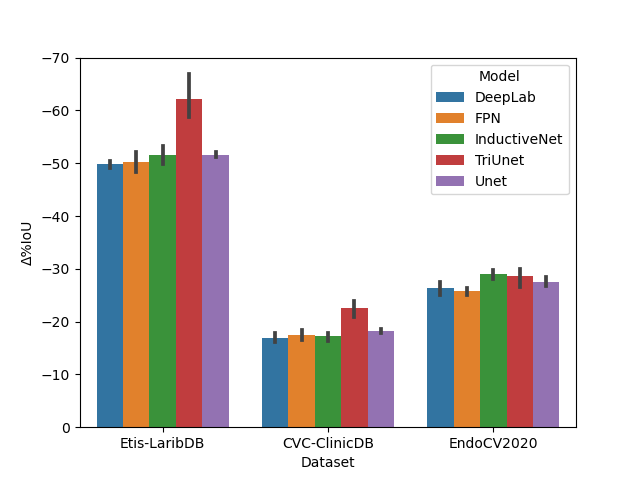
\includegraphics[width=\linewidth]{illustrations/delta_iou_baseline.png}
        \caption{Mean IoUs across models and datasets}
        \label{fig:baseline_ious}
    \end{figure}
    
    All models exhibited comparable performance on Kvasir-Seg, as expected considering ERM. The differences between the models are statistically significant (p>0.xx) even in the \gls{ind} case, however these differences are marginal to the point of being inconsequential for practical purposes. 
    
    The differences become more apparent in \gls{ood} settings, however. Though DeepLabV3+, DD-DeepLabv3+, FPN, and Unet all remain somewhat comparable, albeit with greater margins than in the \gls{ind} case, TriUnet exhibits significant reductions in performance, in particular on Etis-LaribDB. As the TriUnet consists of three Unets, one might expect it to exhibit similar performance to the regular Unet or perhaps even better, but this is evidently not the case. This corroborates the analyses covered in Chapter \ref{background}, which attribute generalization failure to underspecification, which is naturally exacerbated by increased parameter counts. 
    
    \begin{figure}[h]
        \centering
        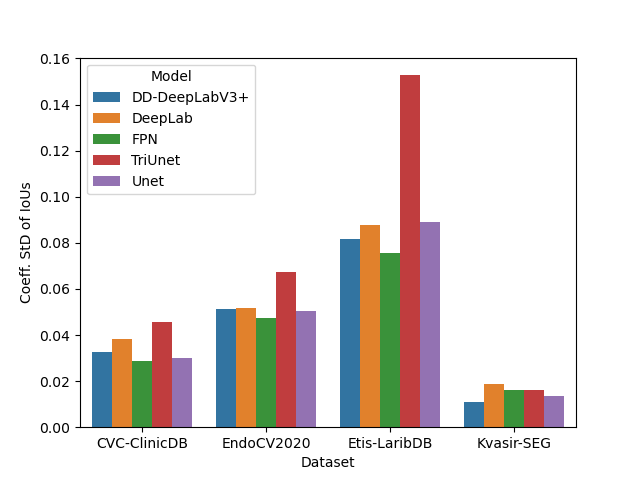
\includegraphics[width=\linewidth]{illustrations/cstd_baseline.png}
        \caption{Coefficient of Standard Deviation across models and datasets}
        \label{fig:baseline_cstd}
    \end{figure}
    
    This is further supported by considering the \gls{cs} across the models. As shown in \autoref{fig:baseline_cstd}, every model exhibits significantly increased variability in its predictions when evaluated on \gls{ood} datasets. When evaluating on the Kvasir-Seg testset, the variability across the ten predictors is practically negligible, with less than a percent in difference regardless of the size or architecture of the model. Moreover, Etis-LaribDB, being the most difficult dataset based on the IoU scores shown in \autoref{fig:baseline_ious}, appears to induce the most variability, which once again supports the findings in \cite{damour2020underspecification}. The TriUnet exhibits the most variability, whereas the regular Unet exhibits fairly stable performance. The UNet, FPN and DD-DeepLabV3+ exhibit increasing variability, inversely correlated with their performance on the respective datasets, as expected. The regular DeepLabV3+, however, exhibits fairly low variability across all the datasets. %TODO: EXPLAIN THIS MYSTERY
    
    
\section{Augmentation Strategies}
The baseline predictors collected in the previous section were then compared to predictors trained using data augmentation. Two augmentation strategies were tested: one with conventional augmentations only, while the other incorporates the GAN-inpainter in addition. The models were trained according to the same hyperparameters as described in \autoref{table:hyperparameters}, and the augmentations were applied with a probability of \(p=0.5\). The results for each configuration and across models and datasets are shown in \autoref{tab:aug_ious}.

\begin{table}[h!]
    \centering
   \begin{tabularx}{\linewidth}{llXr}
\toprule
        \multicolumn{4}{c}{\textbf{Kvasir-SEG}}\\
\toprule
Model & Inpainter + Conventional & None & Conventional\\
\midrule
            DeepLab &  0.846 &  0.818 &  0.852 \\
            FPN &  0.847 &  0.823 &  0.851 \\
           InductiveNet &  0.846 &  0.831 &  0.847 \\
           TriUnet &  0.849 &  0.822 &  0.844 \\
           Unet &  0.842 &  0.828 &  0.850 \\

\toprule
        \multicolumn{4}{c}{\textbf{Etis-LaribDB}}\\
\toprule
Model & Inpainter + Conventional & None & Conventional\\
\midrule
           DeepLab &  0.452 &  0.412 &  0.467 \\
           FPN &  0.427 &  0.403 &  0.439 \\
           InductiveNet &  0.427 &  0.405 &  0.468 \\
           TriUnet &  0.389 &  0.305 &  0.418 \\
           Unet &  0.403 &  0.403 &  0.453 \\
\toprule
        \multicolumn{4}{c}{\textbf{CVC-ClinicDB}}\\
\toprule
Model & Inpainter + Conventional & None & Conventional\\
\midrule
           DeepLab & 0.719 & 0.677 & 0.735 \\
           FPN &  0.703 &  0.677 &  0.716 \\
           InductiveNet &  0.714 &  0.683 &  0.733 \\
           TriUnet &  0.669 &  0.633 &  0.694 \\
           Unet &  0.699 &  0.679 &  0.719 \\
\toprule
        \multicolumn{4}{c}{\textbf{EndoCV2020}}\\
\toprule
Model & Inpainter + Conventional & None & Conventional\\
\midrule
           DeepLab &  0.668 &  0.603 &  0.677 \\
           FPN &  0.665 &  0.604 &  0.662 \\
           InductiveNet &  0.666 &  0.595 &  0.666 \\
           TriUnet &  0.663 &  0.581 &  0.672 \\
           Unet &  0.663 &  0.598 &  0.660 \\
\bottomrule
\end{tabularx}

    \caption{Mean IoUs across augmentation strategies grouped by model and dataset}
    \label{tab:aug_ious}
\end{table}

Both augmentation strategies exhibit an increase in \gls{ood} performance when compared to the baseline (p>0.999). The predictors trained using both conventional augmentations and the inpainter generally perform similarly or worse than the predictors trained with the conventional augmentations only. This is shown in \autoref{fig:augmentations}. There may be several reasons for this: the inpainter may simply not perform well enough to generate believable synthetic images or the GAN may have learned to replicate certain shortcuts in the data and simply strengthen the features that induce generalization failure in the first place.

\begin{figure}
    \centering
    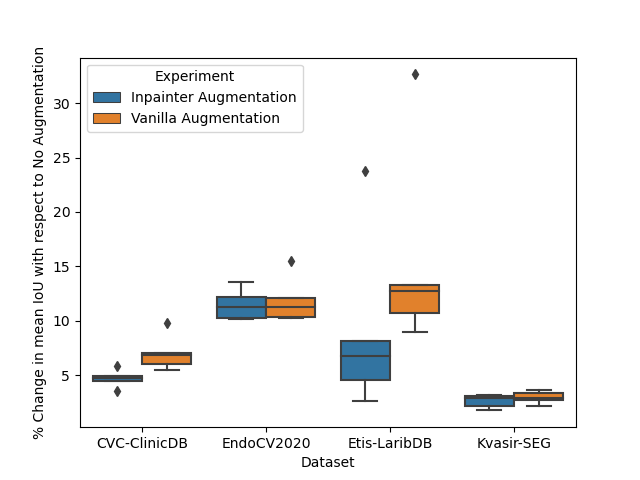
\includegraphics[width=\linewidth]{illustrations/augmentation_plot.png}
    \caption{Bar plot showing overall impact of the respective augmentation strategies, averaged across models}
    \label{fig:augmentations}
\end{figure}

The difference between the three augmentation strategies is particularly well highlighted by the models' performance on Etis-LaribDB, the most difficult of the three \gls{ood} datasets, with performance differences ranging between 10\% and 30\% depending on the model. The differences are slightly less pronounced on the CVC-ClinicDB dataset, and negligible on the two remaining datasets. This does to some extent corroborate the hypothesis that the inpainter has learned dataset-specific shortcuts, as it does not seem to affect the performance in the \gls{ind} case. However, it does not seem to affect the performance on the EndoCV2020 dataset either. 

Regardless, it is clear that synthetic augmentation as implemented in this thesis harms generalization. As will be discussed in \autoref{conclusion}, however, this does not however conclusively prove the inefficacy of \gls{ind}-trained \glspl{gan} for augmentation as a whole. (EXPAND) 


\section{Consistency Training}
Though data augmentation on its own increases generalizability by virtue of the fact that it increases the support of the model, it does not explicitly impose any inductive biases. To address this, Chapter \ref{methods} introduced consistency training. To reiterate, consistency training requires a perturbation model - in practical terms, an augmentation strategy as detailed in the previous section - and a loss function that quantifies the degree to which the model is inconsistent to these perturbations, which for the segmentation task is implemented as \gls{sil}. In the previous section, it was established that conventional augmentations are the most conducive to generalization. Thus, this augmentation strategy was chosen as the perturbation model. 

Ten predictors were trained using consistency training, once again using the same hyperparameters as shown in \autoref{table:hyperparameters}. This was then compared to the predictors trained using the conventional pipeline with the same augmentation strategy. The results are shown in \autoref{tab:aug_ious}. 

\begin{table}[h!]
    \centering
    \begin{tabularx}{\linewidth}{llXX}
    \toprule
    \multicolumn{4}{c}{\textbf{Kvasir-SEG}}\\
    \toprule
    Model & No Augmentation & Conventional Augmentation & Consistency Training\\
    \midrule
        DeepLab & 0.819& 0.853& 0.853 \\
        FPN & 0.823& 0.852& 0.851 \\
        InductiveNet & 0.832& 0.847& 0.853 \\
        TriUnet & 0.822& 0.844& 0.845 \\
        Unet & 0.828& 0.851& 0.851 \\
    \toprule
    \multicolumn{4}{c}{\textbf{Etis-LaribDB}}\\
    \toprule
    Model & No Augmentation & Conventional Augmentation & Consistency Training\\
    \midrule
        DeepLab & 0.412& 0.468& \textbf{0.504} \\
        FPN & 0.404& 0.440& \textbf{0.471} \\
        InductiveNet & 0.406& 0.469& \textbf{0.478} \\
        TriUnet & 0.305& 0.419& \textbf{0.439} \\
        Unet & 0.403& 0.454& \textbf{0.482} \\
    \toprule
    \multicolumn{4}{c}{\textbf{CVC-ClinicDB}}\\
    \toprule
    Model & No Augmentation & Conventional Augmentation & Consistency Training\\
    \midrule
        DeepLab & 0.678& 0.736& 0.740 \\
        FPN & 0.678& 0.717& 0.726 \\
        InductiveNet & 0.683& 0.733& 0.737 \\
        TriUnet & 0.633& 0.695& 0.699 \\
        Unet & 0.679& 0.720& 0.729 \\
    \toprule
    \multicolumn{4}{c}{\textbf{EndoCV2020}}\\
    \toprule
    Model & No Augmentation & Conventional Augmentation & Consistency Training\\
    \midrule
                DeepLab & 0.604& 0.677& 0.678 \\
                FPN & 0.605& 0.663& \textbf{0.674} \\
                InductiveNet & 0.595& 0.667& 0.\textbf{672 }\\
                TriUnet & 0.581& 0.673& \textbf{0.686} \\
                Unet & 0.599& 0.660& \textbf{0.677} \\
    \bottomrule
    \end{tabularx}
    \caption{Mean IoUs for training methods, precision truncated to 95\% confidence. Consistency training entries with greater performance than conventional augmentation by a statistically significant margin (p>0.99) after a one-tailed t-test are highlighted in bold}
    \label{tab:aug_ious}
\end{table}
%decribe more here
\begin{figure}
    \centering
    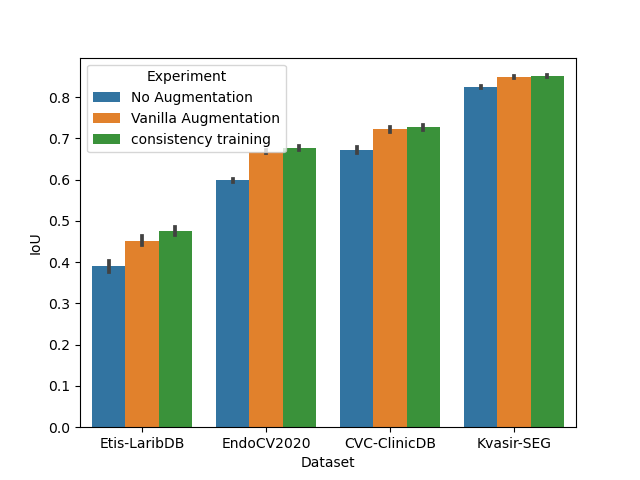
\includegraphics[width=\linewidth]{illustrations/consistency_training_reduced_along_models.png}
    \caption{Effect of training regime averaged across models grouped by dataset}
    \label{fig:consistency_training}
\end{figure}
The results show that consistency training increased generalization when compared to both the baseline and the pipeline with augmentations. The \gls{ood} IoUs were improved by a statistically significant margin for both the Etis-LaribDB dataset and the EndoCV2020 datasets, with p-values of >0.999 and >0.99 respectively. For Kvasir-Seg and CVC-ClinicDB, the differences were statistically insignificant, though this is not necessarily unexpected seeing Kvasir-Seg is \gls{ind} and that the performance gap in CVC-ClinicDB was the smallest of all the datasets. 



\section{Ensemble Generalizability}\label{ensembles}
Finally, the impact of combining multiple predictors into an ensemble was investigated. As the results in previous sections established that consistency training with conventional augmentations exhibited the highest degree of generalizability, it was these predictors that were used in the ensembles. DivergentNet \cite{divergentnets} was also implemented and tested in order to serve as a baseline, with its constituent predictors being trained conventionally and with the same augmentations as used in the previous experiments. 

Two different types of ensembles were compared: combining multiple predictors belonging to the same type of model, and combining multiple predictors each belonging to different models. Both of these approaches were tested in order to evaluate the impact of any potential model-dependent biases with regards to the types of features learned. 

\subsection{Single Model Ensembles}
As mentioned in \autoref{background}, one can consider ensembles - in particular, ensembles consisting of multiple instances of the same model - as bayesian marginalization. To investigate the extent to which this affects generalization, the predictors trained in the last section were assembled into ensembles. All ensembles consisted of four predictors in order to facilitate comparison to DivergentNet, which as mentioned in \autoref{background} exhibited the best performance in EndoCV2021. The predictors were selected randomly from the ten predictors trained for each model in the previous sections. This was then repeated ten times to ascertain statistical significance.

\begin{table}[]
    \centering
    \begin{tabularx}{\linewidth}{lXXXX}
    \toprule
         Model & Kvasir-Seg & Etis-LaribDB & CVC-ClinicDB & EndoCV2020  \\
        \midrule
         DeepLabv3+ &0&0&0&0 \\
         DD-DeepLabv3+ &0&0&0&0 \\
         Unet &0&0&0&0 \\
         TriUnet &0&0&0&0 \\
         FPN &0&0&0&0 \\
         \bottomrule
    \end{tabularx}
    \caption{Caption}
    \label{tab:ensembles}
\end{table}

\autoref{fig:singular_ensemble}
\begin{figure}
    \centering
    \includegraphics[width=\linewidth]{example-image-a}
    \caption{Ensemble Performance }
    \label{fig:singular_ensemble}
\end{figure}



\subsection{Multiple Model Ensembles}
    